\chapter{Моделирование деградации РТГС на основе $Al_{x}Ga_{1−x}As$}
\section{Дуффузионное расплытие активной области}
\begin{figure}[h]
	\centering
	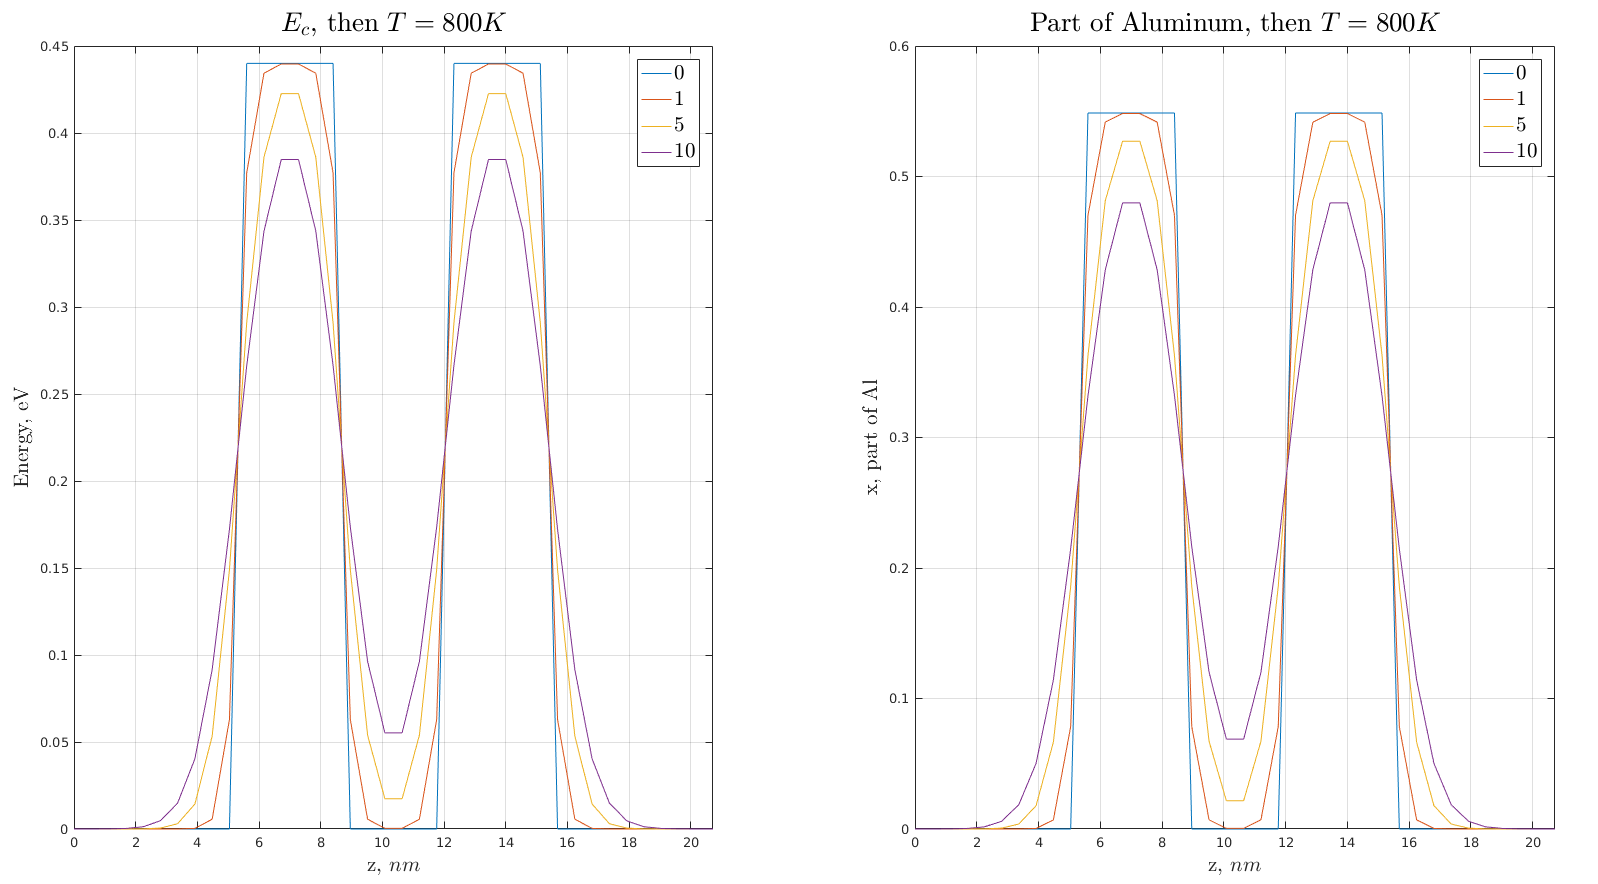
\includegraphics[scale=0.4]{DOAlGaAs}
	\caption{Расплытие потенциального рельефа чистого $Al_{x}Ga_{1−x}As$}
	\label{fig:DOAlGaAs}
\end{figure}

\begin{figure}[h]
	\centering
	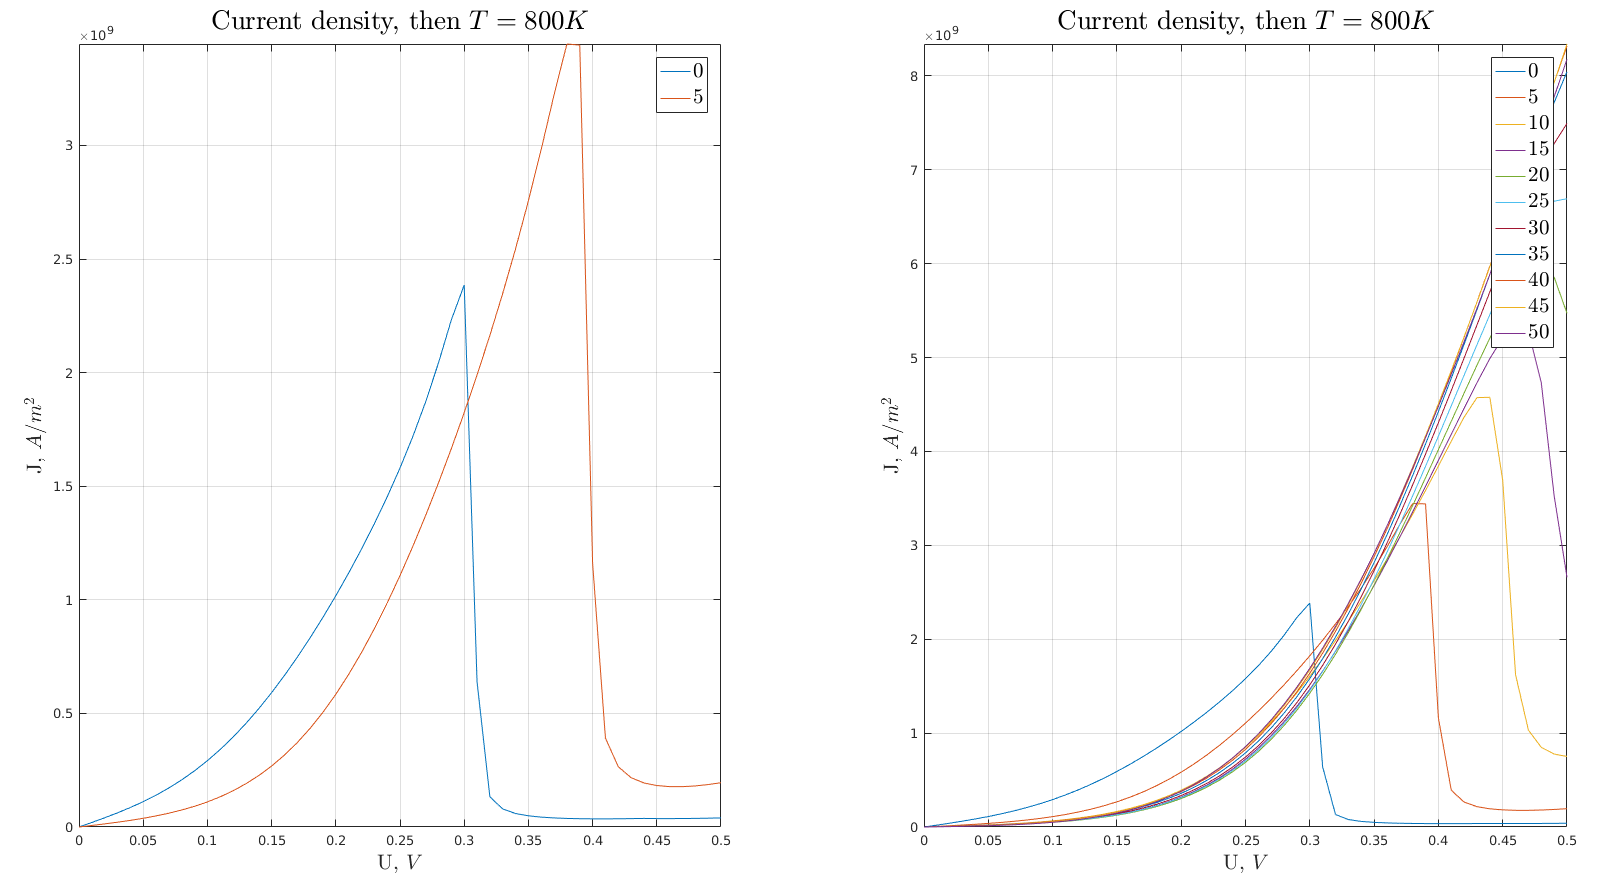
\includegraphics[scale=0.4]{JDOAlGaAs}
	\caption{Деградация тока через РГТС на основе чистого $Al_{x}Ga_{1−x}As$}
	\label{fig:JDOAlGaAs}
\end{figure}

\begin{figure}[h]
	\centering
	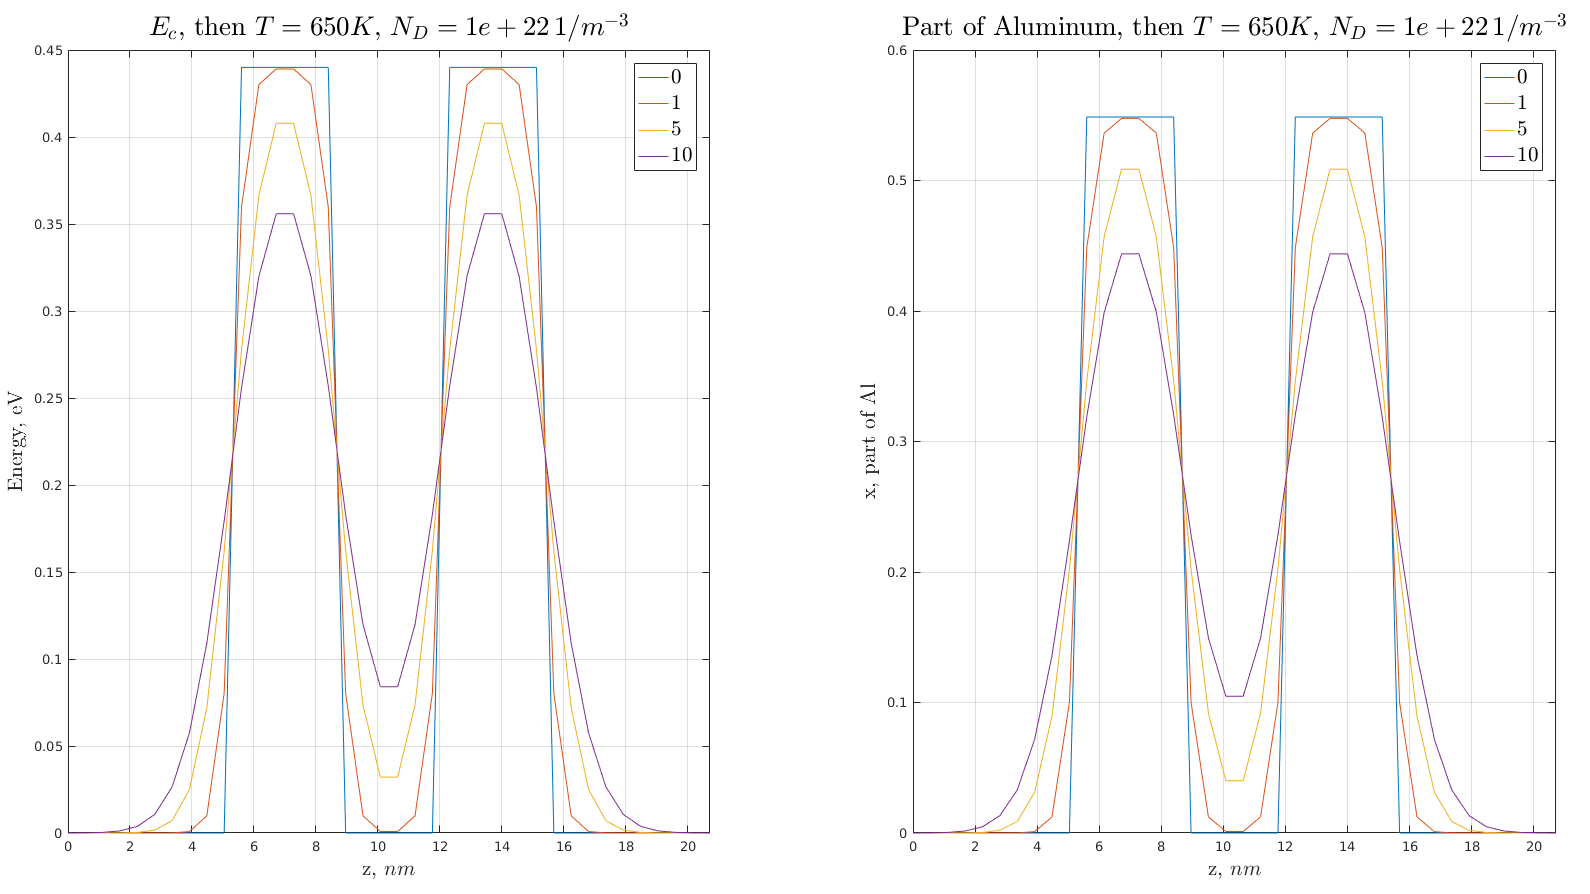
\includegraphics[scale=0.4]{DOAlGaAsNd}
	\caption{Расплытие потенциального рельефа $Al_{x}Ga_{1−x}As$ от диффузии легирующей примеси} 
	\label{fig:DOAlGaAsNd}
\end{figure}

\begin{figure}[h]
	\centering
	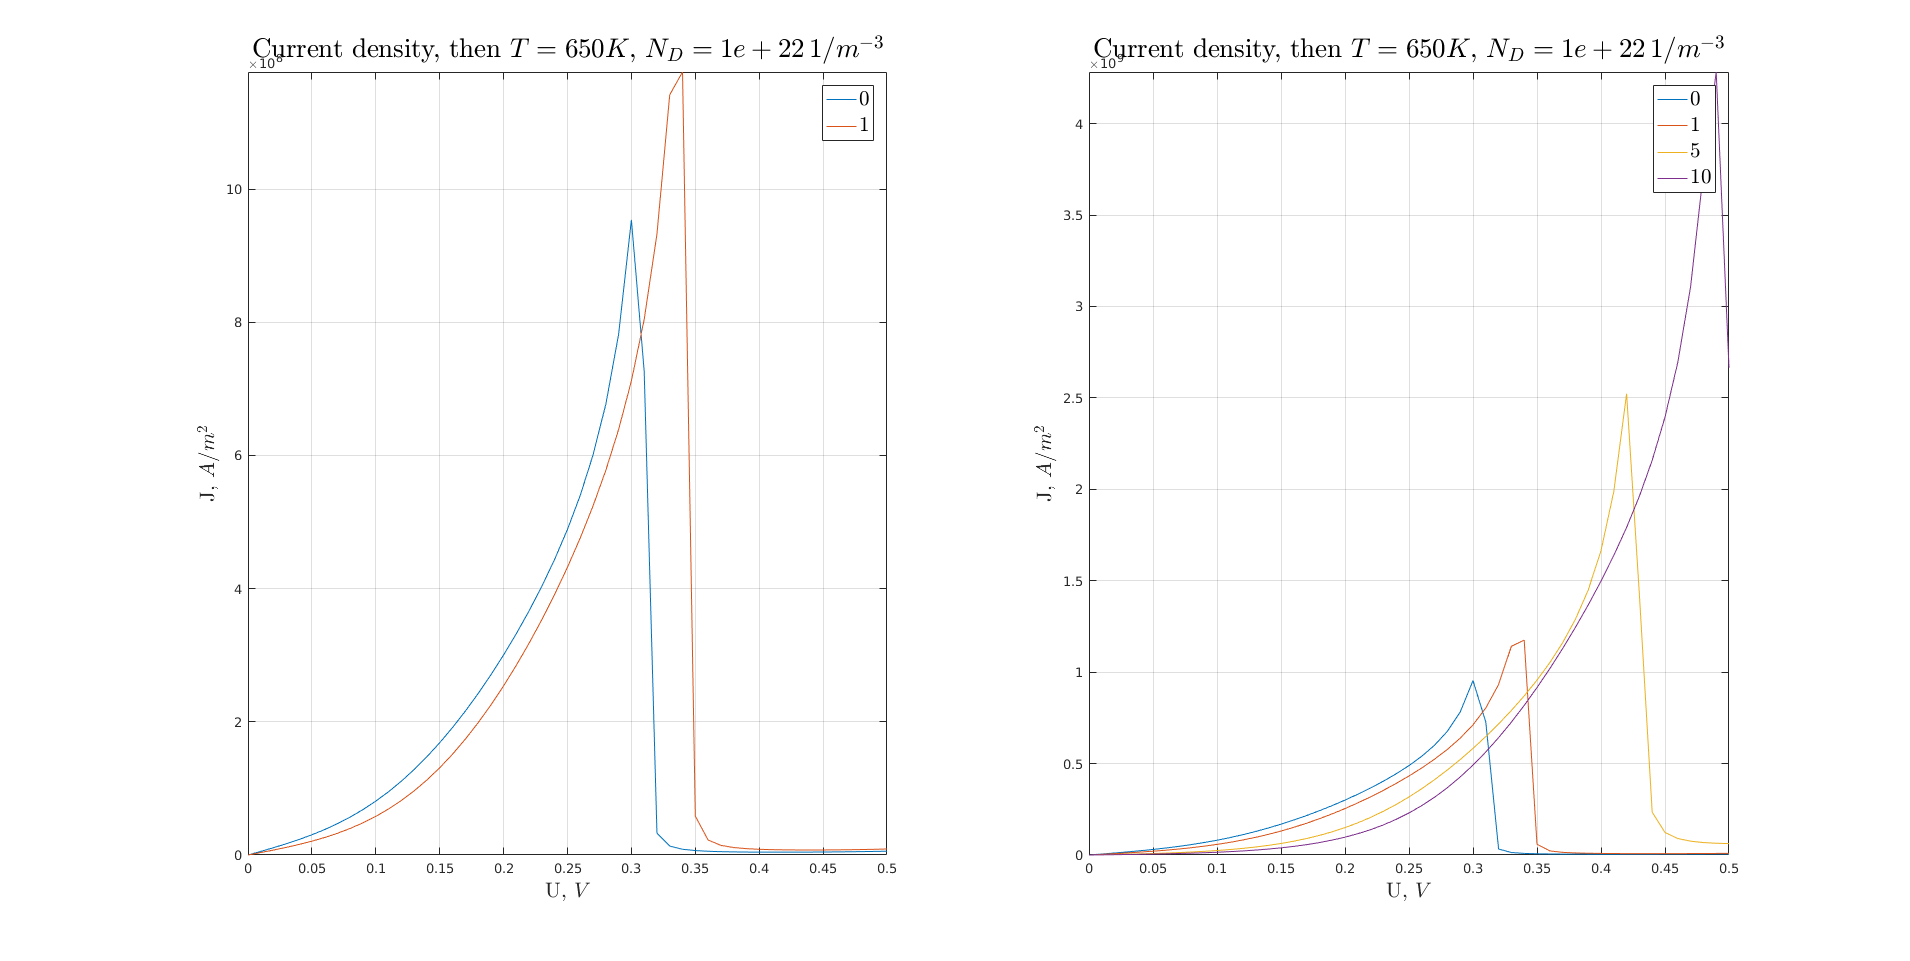
\includegraphics[scale=0.4]{JDOAlGaAsNd}
	\caption{Деградация тока через РГТС на основе $Al_{x}Ga_{1−x}As$ от диффузии легирующей примеси}
	\label{fig:JDOAlGaAsNd}
\end{figure}

\begin{figure}[h]
	\centering
	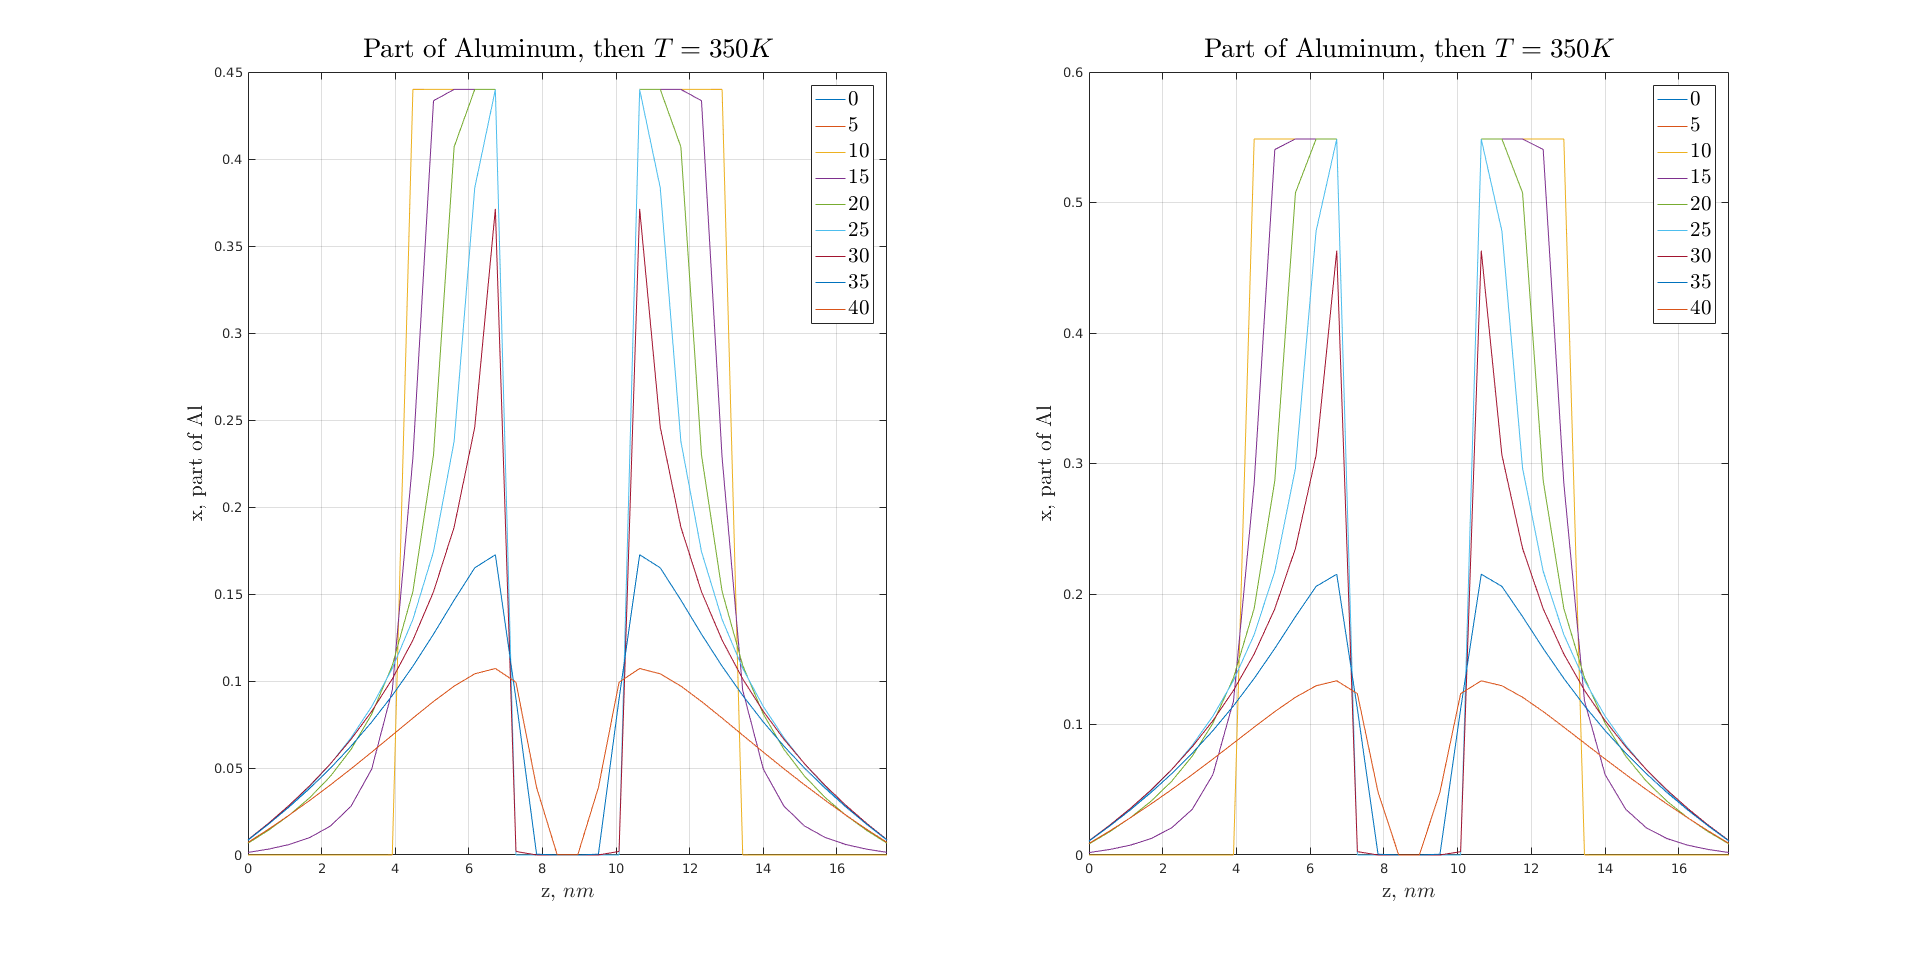
\includegraphics[scale=0.4]{DAlGaAs_Si}
	\caption{Расплытие потенциального рельефа $Al_{x}Ga_{1−x}As$ при наличии донорной примеси} 
	\label{fig:DAlGaAs_Si}
\end{figure}

\begin{figure}[h]
	\centering
	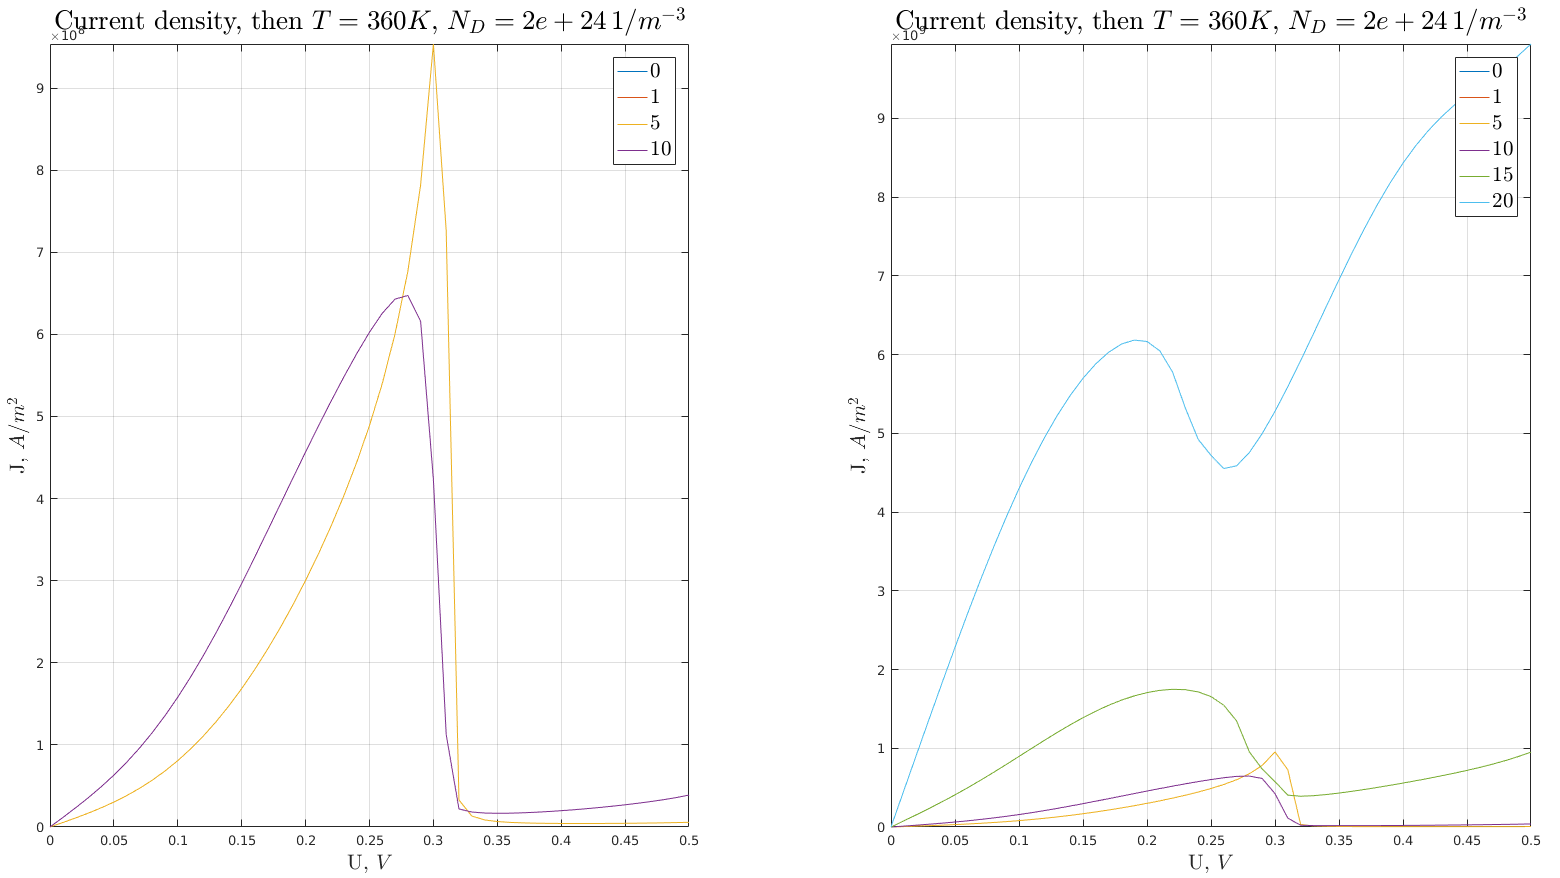
\includegraphics[scale=0.4]{JDAlGaAs_Si}
	\caption{Деградация тока через РГТС на основе $Al_{x}Ga_{1−x}As$ при наличии донорной примеси}
	\label{fig:JDAlGaAs_Si}
\end{figure}